\documentclass[11pt]{article}
\usepackage{fullpage}
\usepackage{hyperref}
\usepackage{listings}
\usepackage{graphicx}
\graphicspath{ {figs/} }

%\usepackage{doublespace}
\begin{document}
\title{Weekly Report - the Ethash Source Code Analysis}
\author{MSc Project \\
Runchao Han \\
}
\maketitle
%
% This section is used to list the key action items from the
% previous meeting. This information will help provide 
% continuity of information and decisions made in the
% previous meeting. 
% Use the \item construct to list each item.  Try to keep the
% descriptions for each down to one or two sentences
%

%TODO references
\section{Progress of the Last Week}

\begin{enumerate}
\item Understood more about Ethash implementations
\item 
\end{enumerate}

\section{Imporing Ethminer to Nvidia Visual Profiler}

The problem I met last two weeks is that I installed two CUDA versions, and the version in \texttt{/bin} is the false one.

After I substituted related binary files with correct ones, the importing succeeded, as shown in Fig.~\ref{fig:nvp}.

\begin{figure}[h]
    \centering
    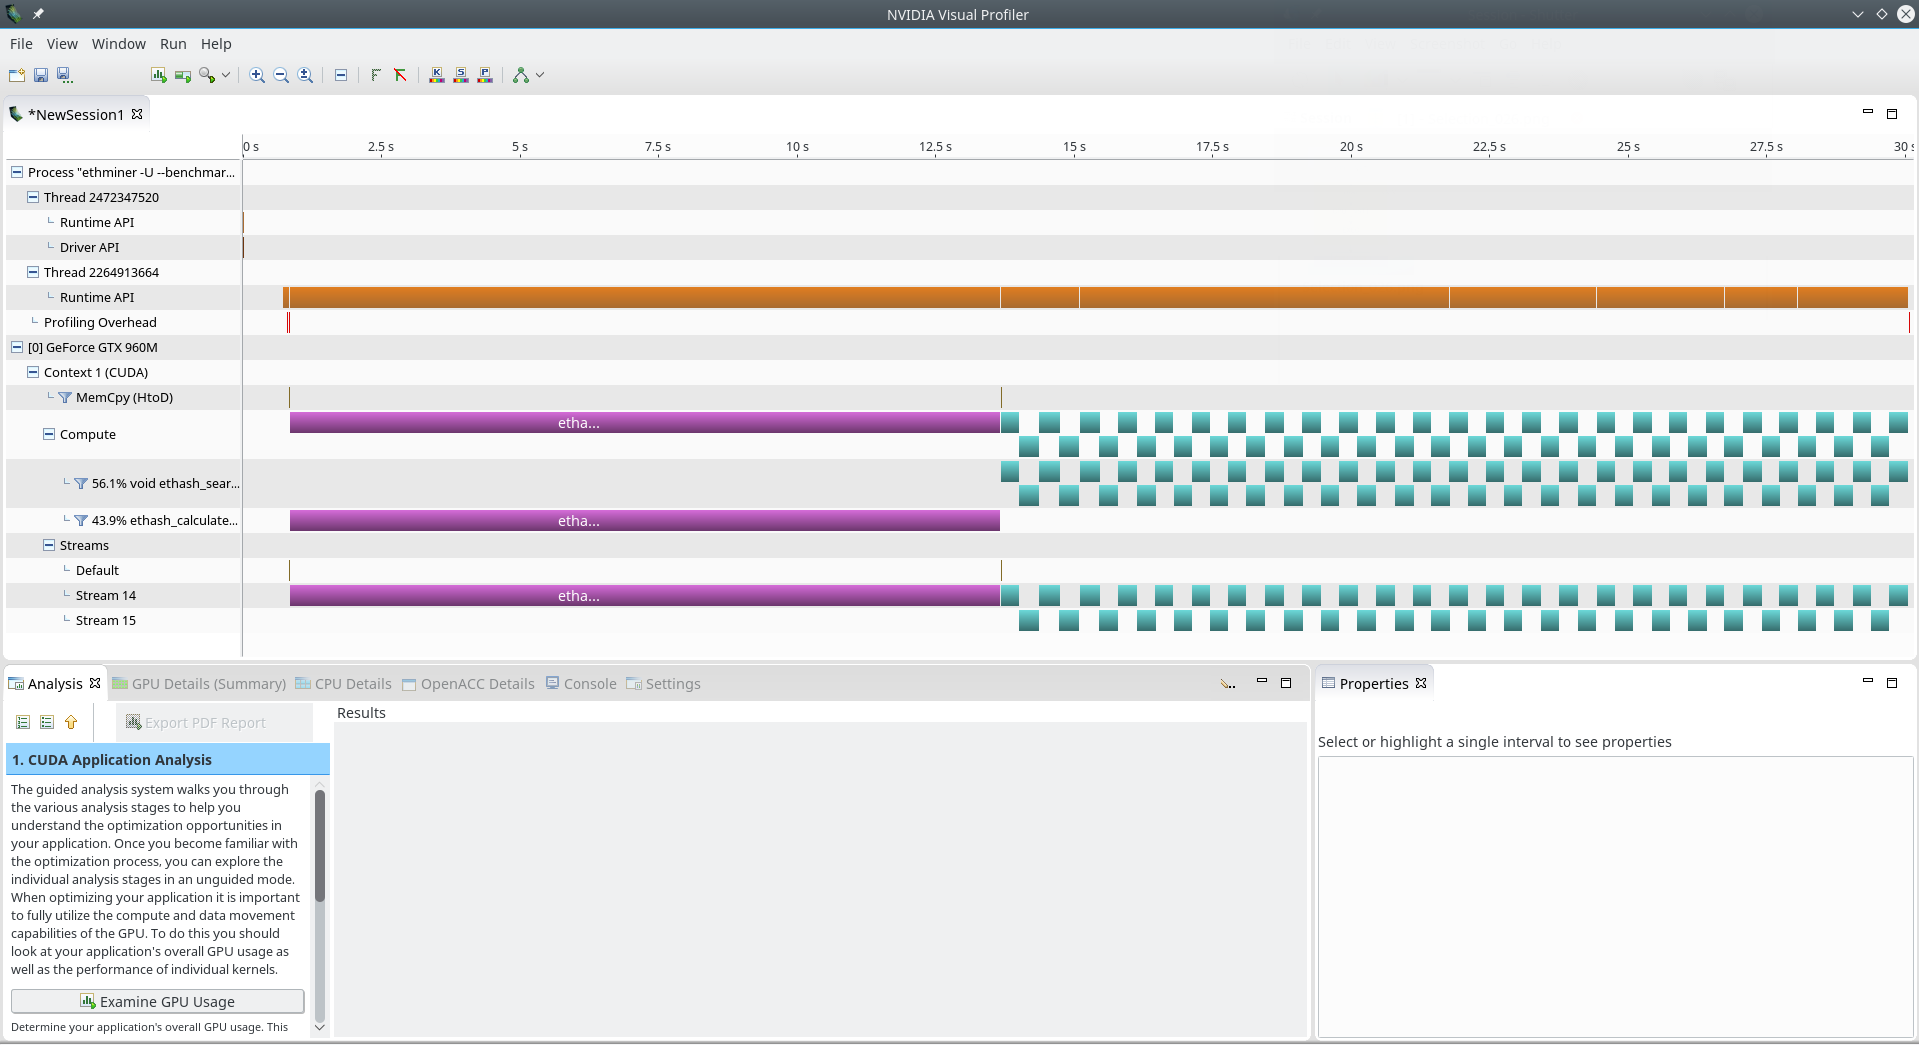
\includegraphics[width=0.8\textwidth]{nvp.eps}
    \caption{Importing the Ethminer to Nvidia Visual Profiler}
    \label{fig:nvp}
\end{figure}

However, this tool is unsuitable for profiling a small part of the code in a big project as far as I know. Before I isolate the critical code from the project, I will still use the timestamp approach.

\section{CUDA Basic Principles}

This two week I spent most time on learning GPU and CUDA, because my hardware knowledge is still rudimentary.

\subsection{An Introduction to GPU}

Graphical Processing Unit (GPU) was designed for computer graphic applications at first, focusing on parallel scientific computing. The comparison between CPU and GPU is shown in Fig.~\ref{fig:gpuvscpu}.

\begin{figure}[h]
    \centering
    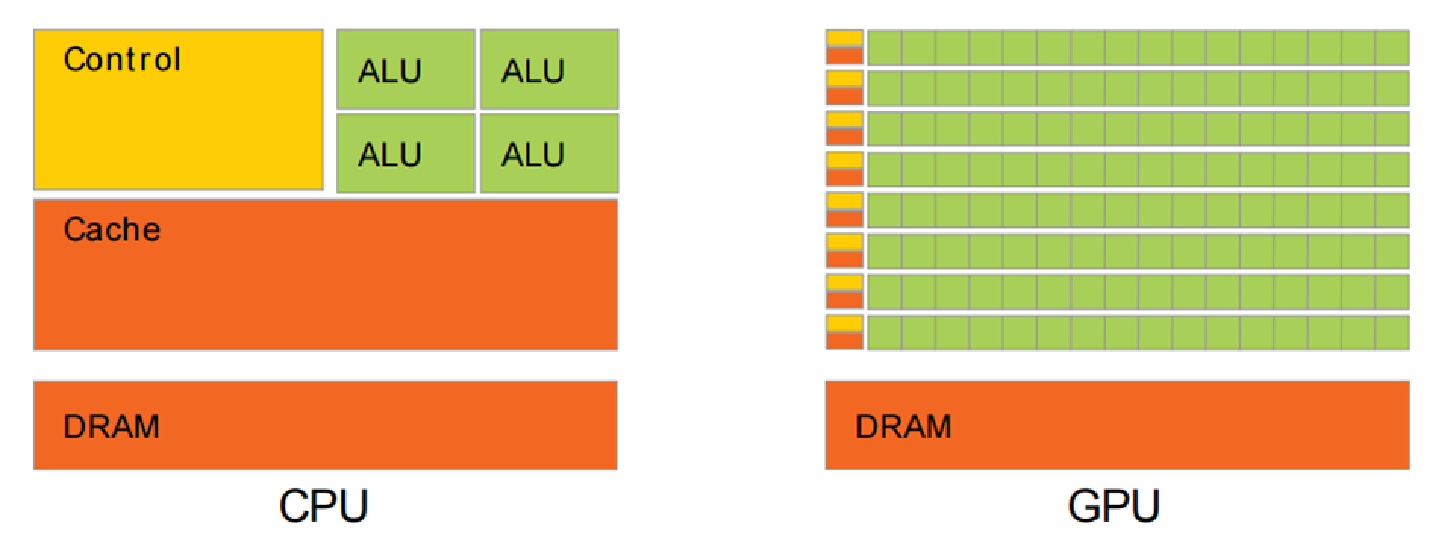
\includegraphics[width=0.8\textwidth]{gpuvscpu.eps}
    \caption{The architecture comparison between CPU and GPU}
    \label{fig:gpuvscpu}
\end{figure}

It is shown that GPU contains much more ALUs which execute computations. Moreover, state-of-the-art GPUs contain a large number of cores so suitable for parallel computing. 

\subsection{The Lifecycle of a CUDA Program}

CUDA was introduced in previous reports, so this section focuses on the execution of a CUDA program.

Fig.~\ref{fig:cuda_exec} shows the logical view of CPU, GPU, main memory and GPU memory.

\begin{figure}[h]
    \centering
    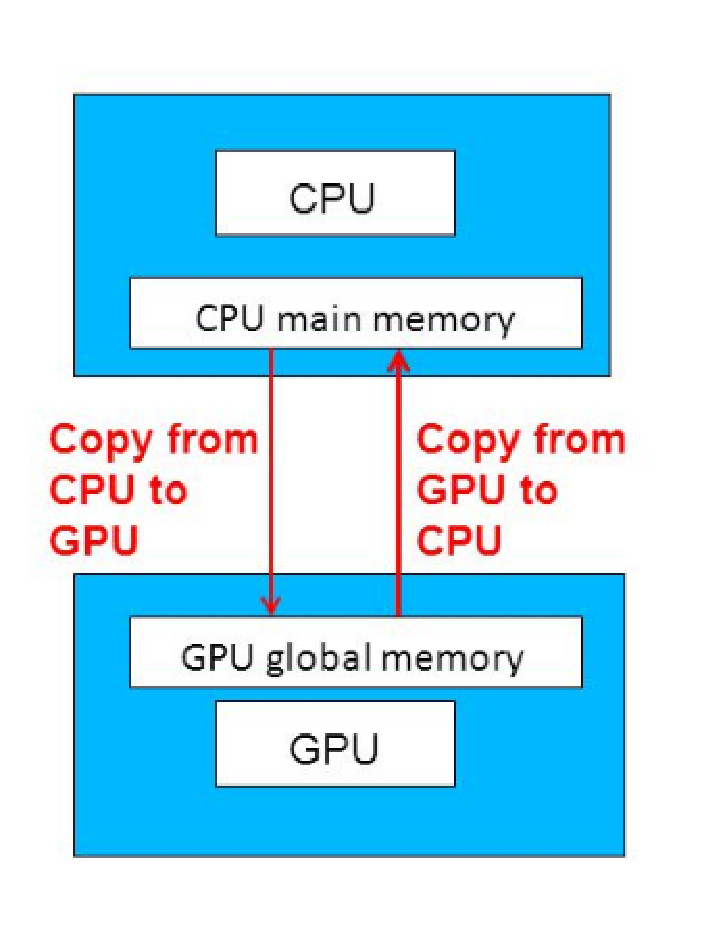
\includegraphics[width=0.8\textwidth]{cuda_exec.eps}
    \caption{The architecture comparison between CPU and GPU}
    \label{fig:cuda_exec}
\end{figure}

A CUDA function is called a ``Kernel function''. 

Typically, a CUDA program is executed by following steps:

\begin{enumerate}
\item Launch the binary file
\item Load data to the main memory
\item Allocate space to data structures in the Graphics Card memory
\item Copy data from the main memory to the Graphics Card memory
\item Invoke the kernel function executed by GPU
\item Copy the result from the Graphics Card memory to the main memory
\end{enumerate}


\subsection{Progammers' Perspective: Grid, Block and Thread}

The concepts of grid, block and thread are on the program level to provide support of organising threads for programmers, as shown in Fig.~\ref{fig:cuda_programmers}. 

\begin{figure}[h]
    \centering
    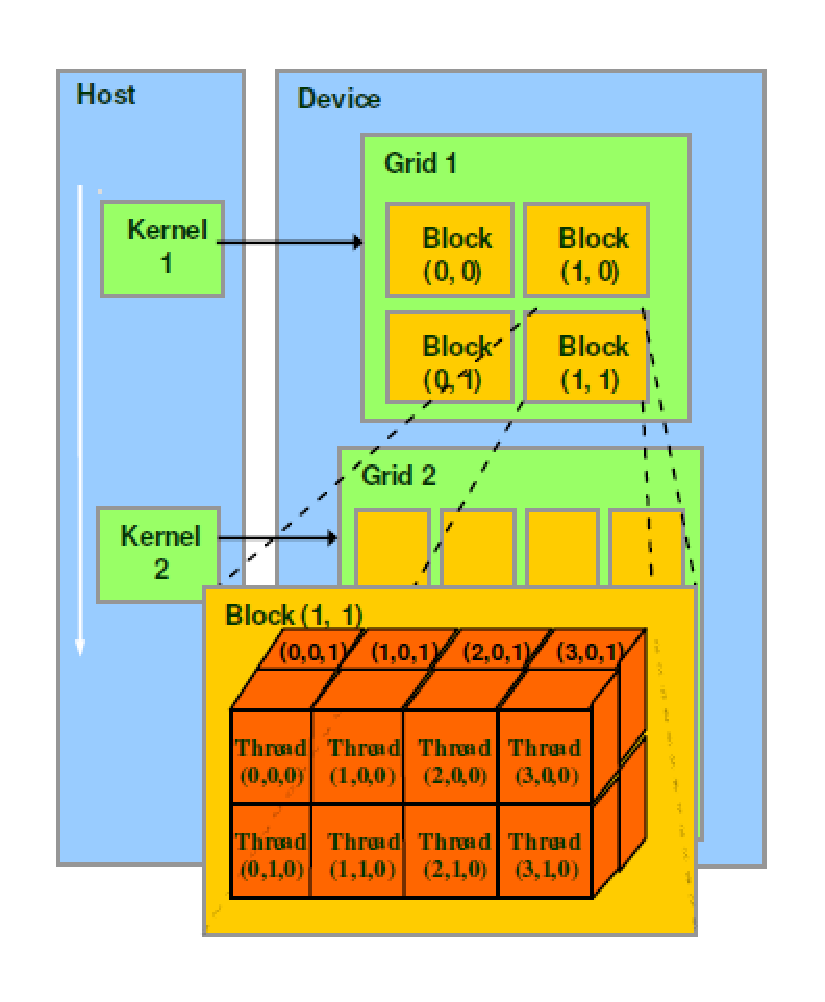
\includegraphics[width=0.8\textwidth]{cuda_programmers.eps}
    \caption{The programmers' perspective of a CUDA program.}
    \label{fig:cuda_programmers}
\end{figure}

A kernel function initialises a grid containing multiple blocks, while a block contains multiple threads. Both blocks and threads are organised as a 3D array.

\subsection{Hardware's Perspective: SP, SM and Warp}

SP means the \texttt{Streaming Processor}, while SM means the \texttt{Streaming Multiprocessor}, the relationship between which is shown in Fig.~\ref{fig:spsm}.

A SP is a core executing instructions, also called CUDA core. SM is a big core consisting of multiple SPs and other resources like registers and warp schedulers, which can be treated as a CPU with multiple cores.

\begin{figure}[h]
    \centering
    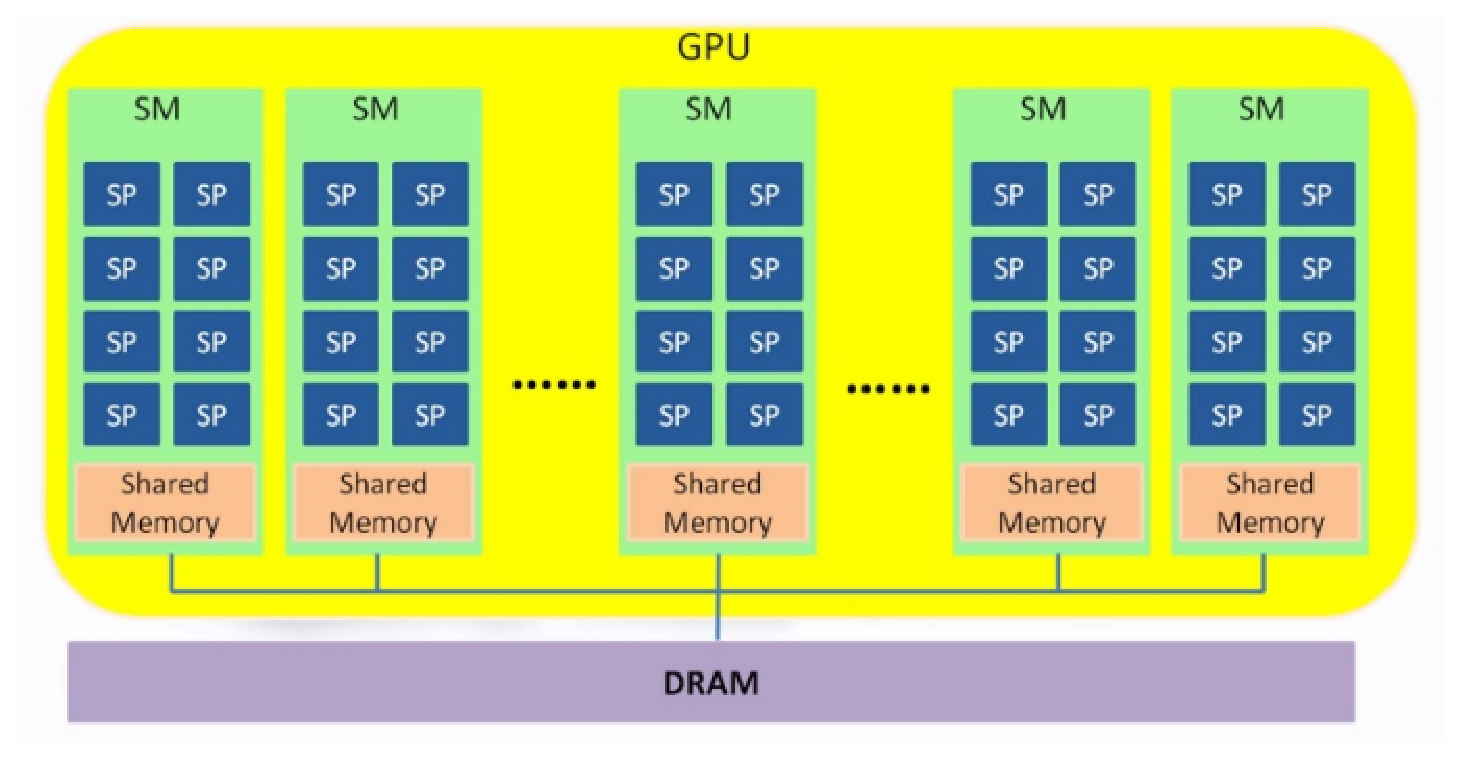
\includegraphics[width=0.8\textwidth]{spsm.eps}
    \caption{The relationship between SP and SM}
    \label{fig:spsm}
\end{figure}

Warp is the basic unit of scheduling containing 32 threads, where 32 threads are executing the same instruction (SIMT). A warp should take a SM to execute, so warps take a SM in turn.

\subsection{Basic APIs}

\subsubsection{Function Type Specifiers}

Function type specifiers specify the execution place of a function, which are:

\begin{itemize}
\item $\_\_device\_\_$: The function is invoked and executed on GPU.
\item $\_\_glocal\_\_$: The function is invoked by CPU and executed on GPU, so called ``Kernel function''.
\item $\_\_host\_\_$: The function is invoked and executed on CPU. This is the default option where the function is a traditional C function.
\end{itemize}

\subsubsection{Variable Type Specifiers}

Variable type specifiers specify the place of variable storage, which are:

\begin{itemize}
\item $\_\_device\_\_$: The data is stored in the Graphical Card memory which every thread can access.
\item $\_\_shared\_\_$: The data is stored in the shared memory in GPU. Only threads in the block can access it.
\item $\_\_constant\_\_$: The data is stored in the constant memory which every thread can access.
\end{itemize}

\subsubsection{Existing Variables}

5 built-in variables in CUDA are used for getting information about the grid, block and thread indices, which are:

\begin{itemize}
\item gridDim: A struct with (x, y, z), which specifies the size of the 3D grid.
\item blockDim: A struct with (x, y, z), which specifies the size of the 3D block.
\item blockIdx: A struct with (x, y, z), which specifies the index of the block of the current thread in the grid
\item threadIdx: A struct with (x, y, z), which specifies the index of the thread of the current thread in the block
\item warpSize: The size of the warp. (Compute Capability>1.0?32:24)
\end{itemize}

\subsection{The New Shuffle APIs}

In the newest CUDA version 9.0, the Shuffle APIs are created. $\_\_shfl()$ is used for exchanging variables among threads in a warp. Compared to the conventional shared memory, Shuffle can do the same thing with the better efficiency. More information can be found at \footnote{https://people.maths.ox.ac.uk/gilesm/cuda/lecs/lec4.pdf}.

Ethash is implemented by both ways: the shared memory and the Shuffle. I just have figured out CUDA basics so I only tested the Shuffle implementation.

\section{A More Detailed Profiling on Ethash (Shuffled)}

This time I did a detailed profiling, but still haven't figured out the implementation because of CUDA (Now it is much better). I uploaded my data and my Jupyter notebook to Github.\footnote{https://github.com/SebastianElvis/MScProject/tree/master/tests/Ethash\textunderscore tests}

However I haven't draw a stack graph, because the data is still coarse grained and some parts take time much longer than other parts, making the graph hard to read.

\section{Miscellaneous}

%
% This section is used to list the following week's plan
% Use the \item construct to list each item.  Try to keep the
% Descriptions for each down to one or two sentences
%
\section{Next Week's Plan}
\begin{enumerate}
\item Figure out the Ethash code and comment on every line
\item Output an analysis of the Ethash source code
\end{enumerate}


%\bibliographystyle{plain}
%\bibliography{references.bib}

\end{document}
